\section{Détection de contours et extraction de lignes}

\subsection{Détection de contours}

La première étape de notre processus de reconnaissance de grillage est de détecter les contours d'une image. En effet, les grillages provoquent naturellement une notion de contour dans l'image de par leur superposition sur le paysage.

Il existe de nombreuses manières d'obtenir un détecteur de contours, nous avons opté pour la méthode de Canny. Celle-ci a l'avantage de procéder par seuillage par hysteresis ce qui permet d'obtenir de bons résultats - au prix d'une recherche des paramètres optimaux.

Le filtre de Canny commence par un filtrage avec un noyau Gaussien dont la variance détermine l'échelle de précision. Celle-ci doit être en accord avec la taille du grillage pour que ce dernier provoque des contours intéressants. Il y a donc deux possibilités :
\begin{enumerate}
\item adapter variance de la gaussienne à la taille caractéristique du grillage. Cette méthode nécessite d'avoir une connaissance \emph{a priori} de la taille du grillage et n'est donc pas satisfaisante en pratique - dans un cas purement non supervisé où l'on en souhaite pas d'intervention extérieure donnant cette taille ;
\item redimensionner les images pour que les grillages aient une taille - à peu près - fixe entre plusieurs images. Ceci repose sur l'hypothèse que les grillages ont grossièrement la même largeur dans chaque image. C'est bien sûr illusoire, mais de manière sous-jacente ceci implique qu'il n'y a pas de grillage qui recouvre la moitié de l'image et d'autres quasi-invisibles. Notons que ce redimensionnement sera nécessaire quoiqu'il arrive lors de l'\emph{inpainting}.
\end{enumerate}

Les résultats de détecteur de contours sont fournis en Fig.(\ref{fig101}). On voit qu'ils sont plutôt bons dans le sens où le grillage est presque partout visible dans les contours. Comme c'est cette information qui est ensuite envoyée pour en extraire les lignes, il est primordial que les lignes soient bien représentées.

\begin{figure}[ht!]
\centering
\begin{tabular}{cc}
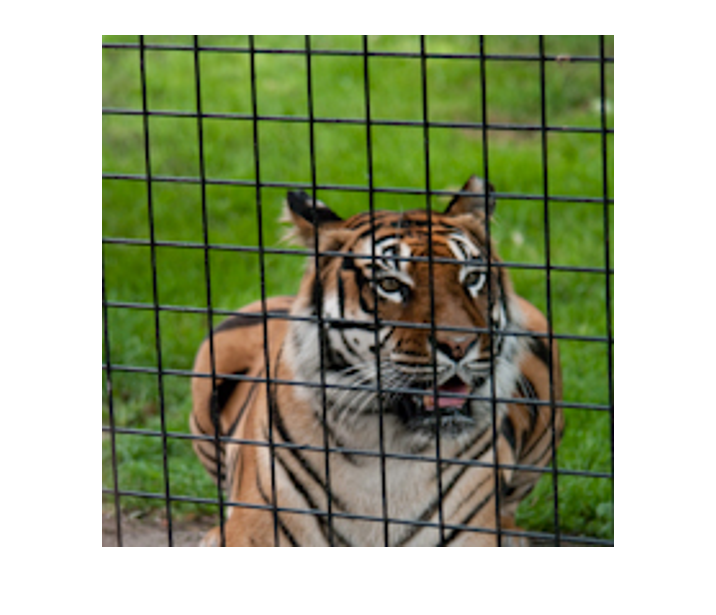
\includegraphics[width = .5\columnwidth]{fig/tigre_rescale.png} &
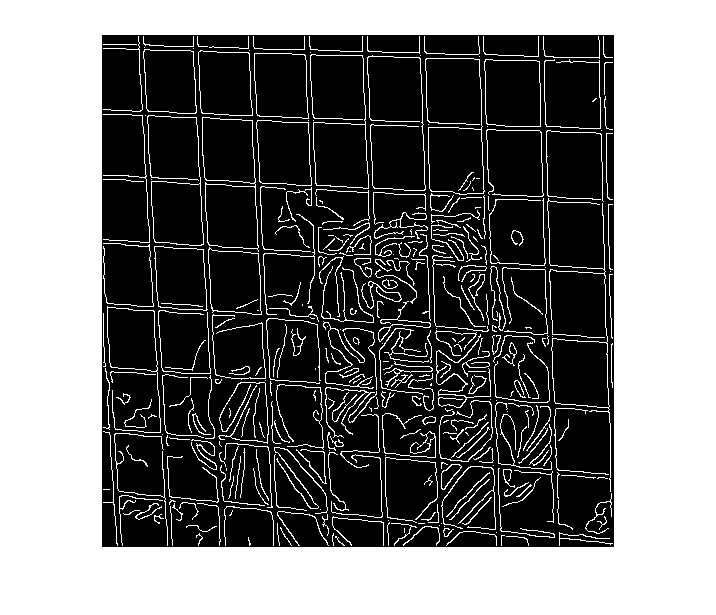
\includegraphics[width = .5\columnwidth]{fig/contour.png} \\
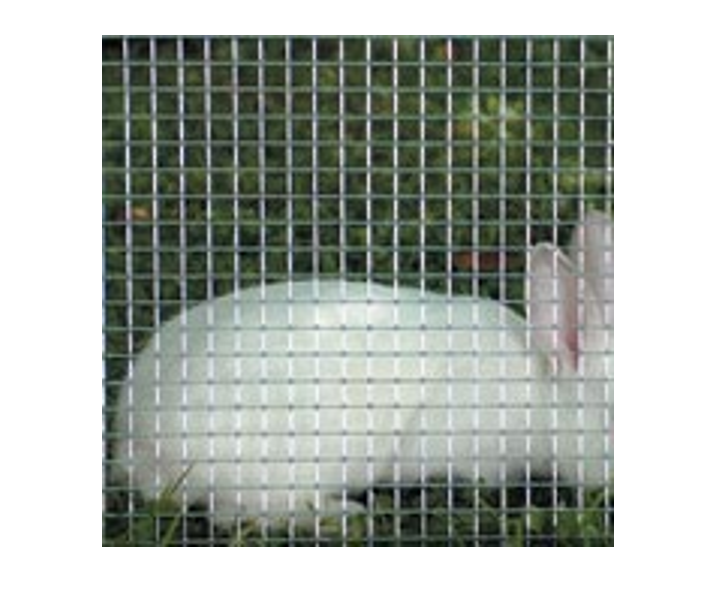
\includegraphics[width = .5\columnwidth]{fig/lapin_rescale.png} &
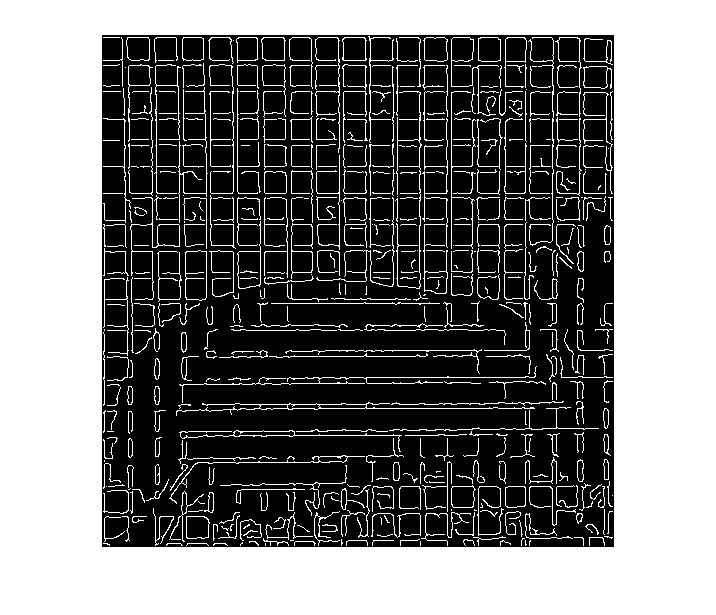
\includegraphics[width = .5\columnwidth]{fig/contour_lapin.png} \\
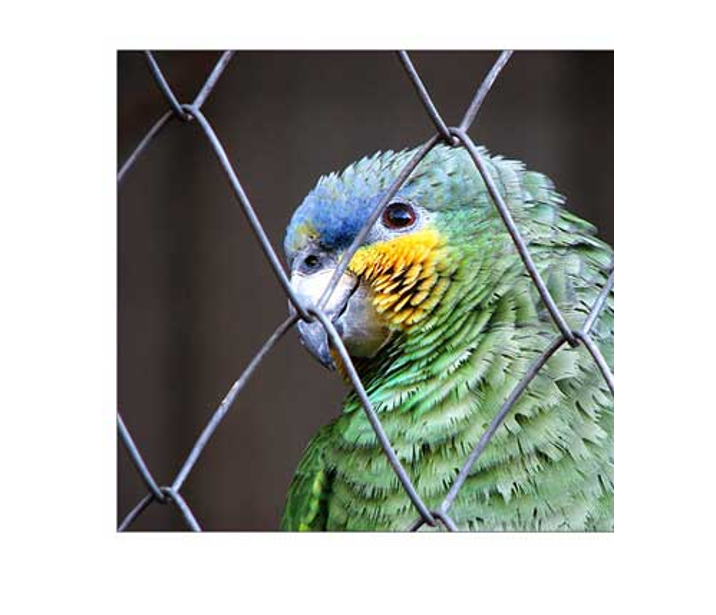
\includegraphics[width = .5\columnwidth]{fig/parrot_rescale.png} &
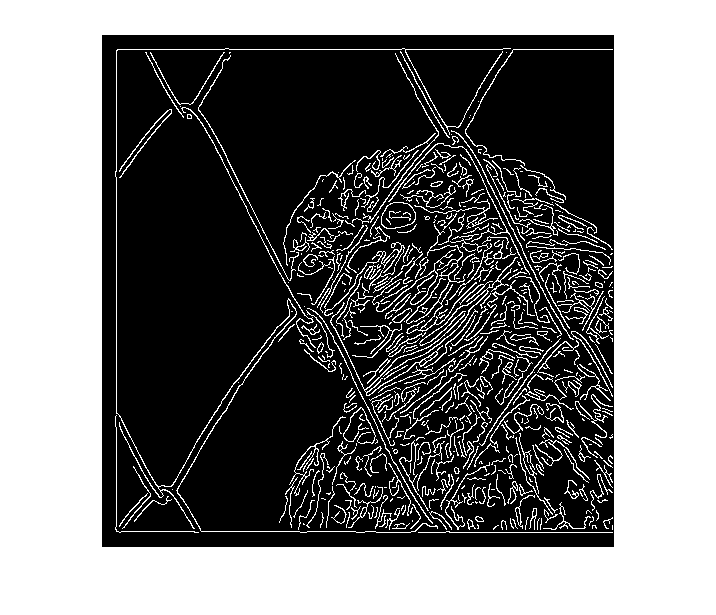
\includegraphics[width = .5\columnwidth]{fig/contour_parrot.png}
\end{tabular}
\caption{Dans les colonnes de gauche, l'image initiale et dans celles de droite les résultats de la détection de contour avec l'algorithme de Canny. Toutes les images sont redimensionnées en $512\times 512$. }
\label{fig101}
\end{figure}

\subsection{Extraction de lignes - transformation de Hough}

Nous ne rentrons pas dans les détails de la transformation de Hough mais en donnons ici plus une intuition qui nous sera utile pour plus tard. La transformation de Hough est une transformation qui permet d'extraire des droites d'une image. Le processus est représenté de manière graphique en Fig.(\ref{fig102}).

L'idée est de partir d'un point $A$ et de considérer toutes les droites passant par ce point. Ces droites sont paramétrées en coordonnées $(\rho,\theta)$ représentant respectivement l'angle et la distance - notons que sur un ordinateur, le point (0,0) est en haut à gauche et non en bas à gauche :
\begin{equation}
r = x \cos \theta + y \sin\theta
\end{equation}
Les droites passant par $A$ forment une sinusoïde dans l'espace d'arrivée. La droite passant par $A$ qui va passer par un autre point $B$ va également appartenir à la sinusoïde de $B$ dans l'espace image : elle sera représentée par un point à l'intersection des deux sinusoïdes. Pareil si cette même droite passe par un point $C$. C'est ainsi que si l'on alloue un compteur 1 à chaque sinusoïde d'un ensemble de points d'entrée, et que ce compteur est additif, alors trouver les maxima dans la transformation de Hough revient effectivement à extraire les lignes d'un nuage de points.

\begin{figure}[ht!]
\centering
\begin{tabular}{cc}
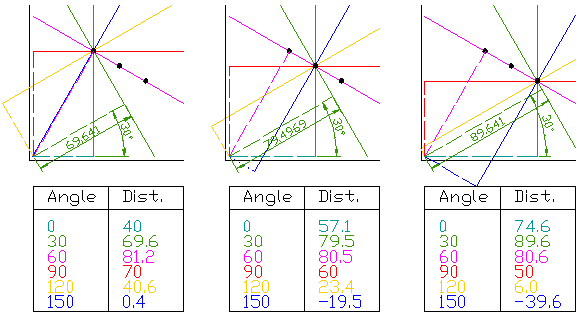
\includegraphics[width = .5\columnwidth]{fig/Hough_transform_diagram.png} &
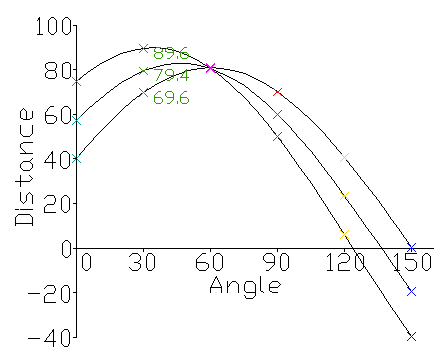
\includegraphics[width = .5\columnwidth]{fig/Hough_space_plot_example.png}
\end{tabular}
\caption{Transformation de Hough, les croisements dans l'espace arrivé correspondent aux droites dans l'image initiale. }
\label{fig102}
\end{figure}



